\documentclass[runningheads]{llncs}

% ---------------------------------------------------------------
% Include basic ECCV package
 
% TODO REVIEW: Insert your submission number below by replacing '*****'
% TODO FINAL: Comment out the following line for the camera-ready version
\usepackage[review,year=2026,ID=*****]{eccv}
% TODO FINAL: Un-comment the following line for the camera-ready version
%\usepackage{eccv}

% OPTIONAL: Un-comment the following line for a version which is easier to read
% on small portrait-orientation screens (e.g., mobile phones, or beside other windows)
%\usepackage[mobile]{eccv}


% ---------------------------------------------------------------
% Other packages

% Commonly used abbreviations (\eg, \ie, \etc, \cf, \etal, etc.)
\usepackage{eccvabbrv}

% Include other packages here, before hyperref.
\usepackage{graphicx}
\usepackage{booktabs}
\usepackage{placeins}

% The "axessiblity" package can be found at: https://ctan.org/pkg/axessibility?lang=en
\usepackage[accsupp]{axessibility}  % Improves PDF readability for those with disabilities.


% ---------------------------------------------------------------
% Hyperref package

% It is strongly recommended to use hyperref, especially for the review version.
% Please disable hyperref *only* if you encounter grave issues.
% hyperref with option pagebackref eases the reviewers' job, but should be disabled for the final version.
%
% If you comment hyperref and then uncomment it, you should delete
% main.aux before re-running LaTeX.
% (Or just hit 'q' on the first LaTeX run, let it finish, and you
%  should be clear).

% TODO FINAL: Comment out the following line for the camera-ready version
%\usepackage[pagebackref,breaklinks,colorlinks,citecolor=eccvblue]{hyperref}
% TODO FINAL: Un-comment the following line for the camera-ready version
\usepackage{hyperref}

% Support for ORCID icon
\usepackage{orcidlink}


\begin{document}

% ---------------------------------------------------------------
% TODO REVIEW: Replace with your title
\title{RefCompose: Multi-Reference Image Generation via LoRA-Conditioned Diffusion} 

% TODO REVIEW: If the paper title is too long for the running head, you can set
% an abbreviated paper title here. If not, comment out.
\titlerunning{Abbreviated paper title}

% TODO FINAL: Replace with your author list. 
% Include the authors' OCRID for the camera-ready version, if at all possible.
\author{First Author\inst{1}\orcidlink{0000-1111-2222-3333} \and
Second Author\inst{2,3}\orcidlink{1111-2222-3333-4444} \and
Third Author\inst{3}\orcidlink{2222--3333-4444-5555}}

% TODO FINAL: Replace with an abbreviated list of authors.
\authorrunning{F.~Author et al.}
% First names are abbreviated in the running head.
% If there are more than two authors, 'et al.' is used.

% TODO FINAL: Replace with your institution list.
\institute{Princeton University, Princeton NJ 08544, USA \and
Springer Heidelberg, Tiergartenstr.~17, 69121 Heidelberg, Germany
\email{lncs@springer.com}\\
\url{http://www.springer.com/gp/computer-science/lncs} \and
ABC Institute, Rupert-Karls-University Heidelberg, Heidelberg, Germany\\
\email{\{abc,lncs\}@uni-heidelberg.de}}

\maketitle


\begin{abstract}

Filmmakers and visual artists routinely need to compose multiple references, actors, locations, props, cultural elements, into a single coherent shot, but existing tools either fail to scale past a handful of references or destroy fine grained subject identity in the process. This stems from two compounding limitations: per reference tokenization scales memory linearly with reference count $N$, and existing methods fail to faithfully preserve the appearance of each reference subject, producing generated content that departs from the given reference images rather than reproducing them. We propose \textbf{RefCompose}, a pixel space compositional conditioning framework that decouples \emph{where} things go from \emph{what} they look like. RefCompose builds a single fixed resolution reference canvas that keeps conditioning size constant regardless of reference count, with spatial layout induced at inference time from a frozen diffusion transformer and extracted via Grounding DINO, requiring no LLM or dedicated layout model. Dual stream LoRA adapters then inject a layout derived depth map and the encoded canvas through separate low rank streams, disentangling geometric scaffolding from localized appearance. Benchmarked against both layout based and state of the art multi reference generation methods on the Dense Layout protocol, RefCompose consistently outperforms these baselines across color, texture, shape, and spatial accuracy, as well as identity and content preservation metrics at higher reference counts, all with constant inference memory regardless of reference count, making it a practical building block for multi subject cinematic composition at production scale.
  \keywords{Diffusion Models \and Image Generation \and LoRA}
\end{abstract}


\section{Introduction}
\label{sec:intro}




Controllable image synthesis has emerged as a central challenge in modern generative modelling, with applications spanning advertising, cinematic pre-visualisation, and synthetic data production. 
In the context of movie concept generation using text-to-image (T2I) diffusion models, a single composite frame serves as the critical blueprint across various stages of production, bridging abstract concepts and final visual execution. This visual reference must faithfully reproduce the appearance of specific actors, real-world locations, cultural aesthetics, and narrative objects~\cite{wu2025uno,xverse2024,wang2024msdiffusion,omnigen2_2025}.

Existing T2I methods face significant limitations when textual prompts are the sole control signal. Text prompts often require iterative refinement to encode texture, identity, and style simultaneously across multiple subjects; yet arriving at a prompt that reliably captures all these attributes under heterogeneous data conditions remains a non-trivial challenge. Furthermore, pretrained models underrepresent certain concepts (e.g., cultural), leaving gaps in the common vocabulary due to inherent bias in the training data distribution. This gap undermines the composite image generation through text alone and limits the broader applicability of controllable image generation. Layout-to-Image generative models~\cite{feng2024layoutgpt,li2023gligen,xiang2025instanceassemble,tang2024creatilayout,lian2023layoutdiffusion} use bounding-box layouts to pair spatial coordinates with localized prompts alongside a global prompt. However, these sparse region-level descriptions still fail to reconstruct intended appearances under complex occlusion scenarios faithfully. These challenges highlight that dense visual instance cues provide reliable multimodal content, ensuring subject alignment, positioning, and preserving semantic attributes in composite image generation.


\begin{figure}[t]
\centering
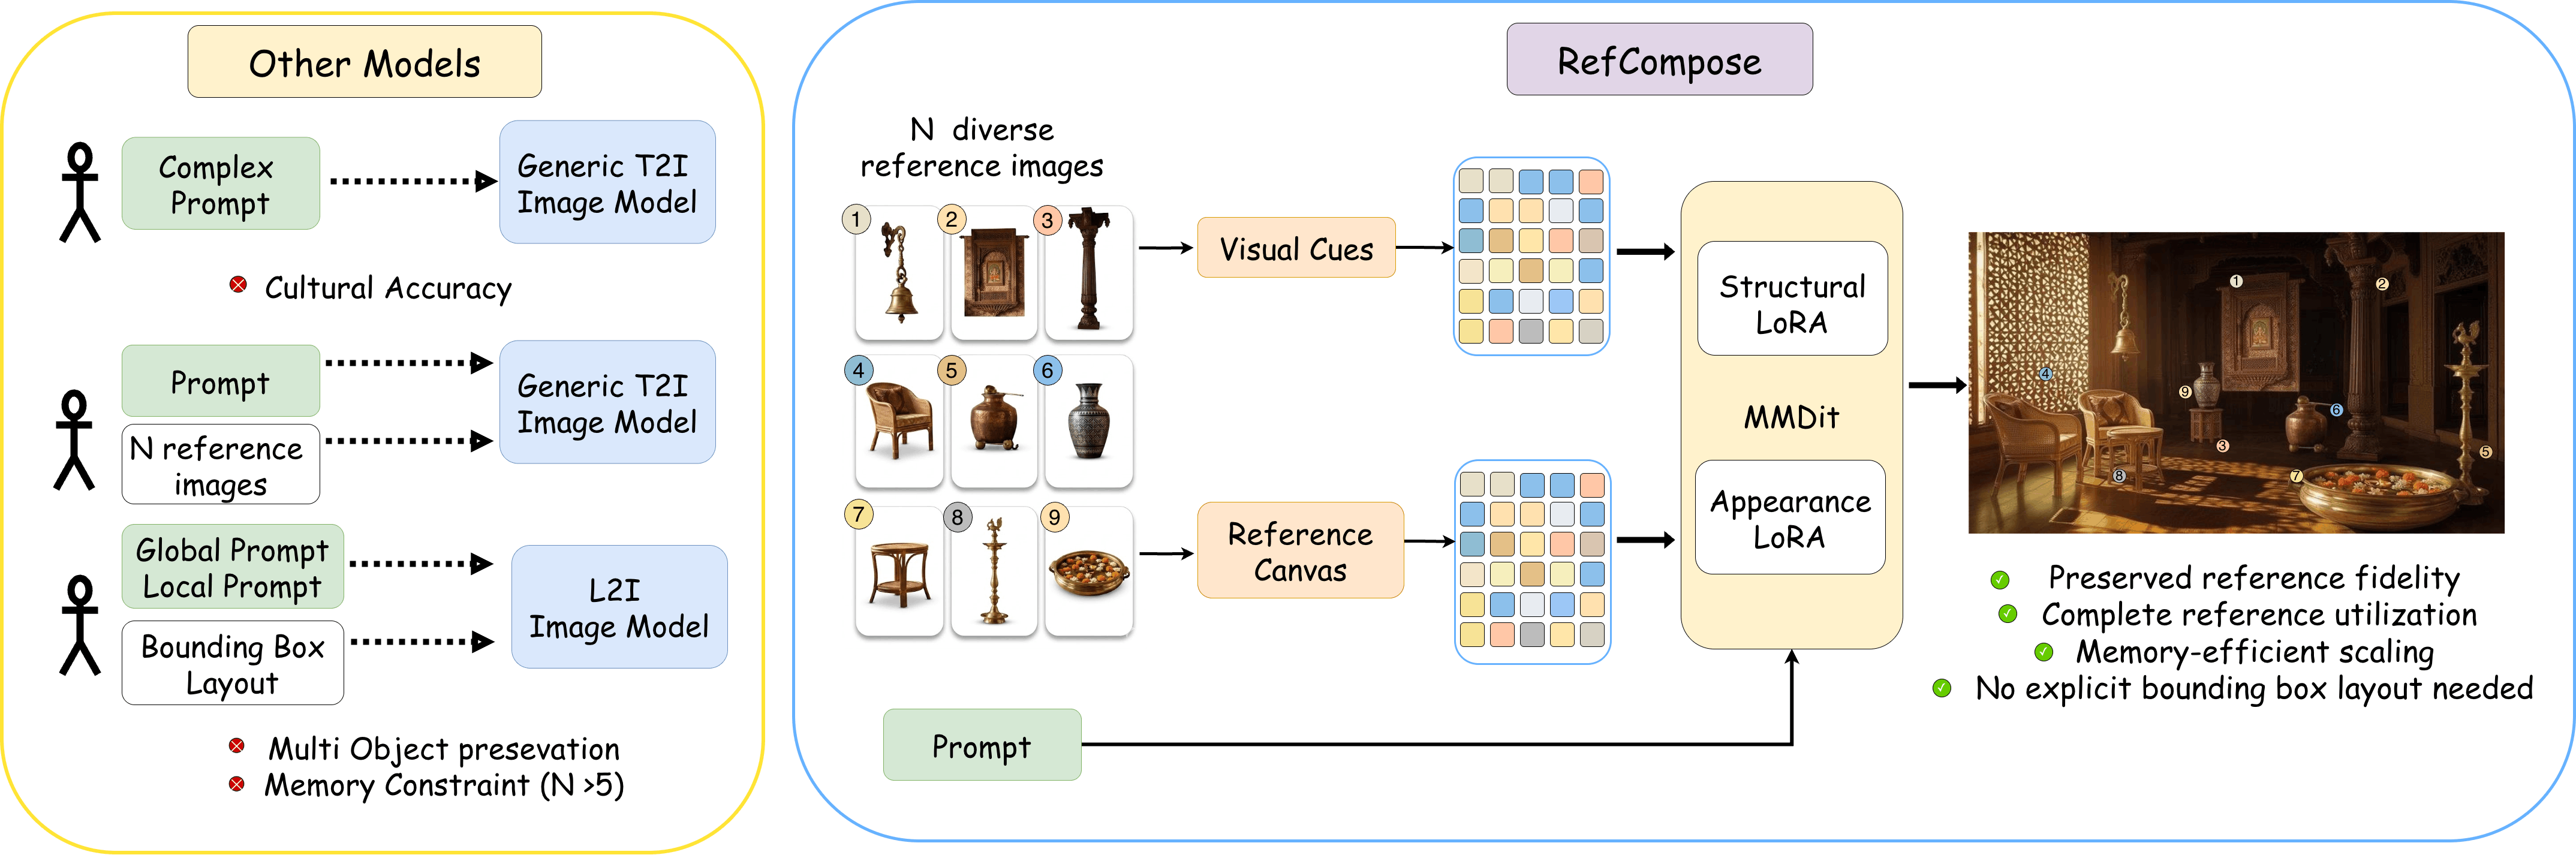
\includegraphics[width=\linewidth]{images/final_abstract_compressed.png}
\caption{Conceptual comparison between prior multi-reference generation paradigms and RefCompose. Existing approaches suffer from memory overhead scaling linearly with reference count, cultural fidelity gaps, or inability to preserve subject appearance without bounding-box supervision. RefCompose resolves these limitations via 1. a fixed-resolution reference canvas encoding arbitrary references at constant token cost, and 2.  layout from dense visual cues induced directly from a structured text prompt.}
\label{fig:conceptdiagram}
\end{figure}


Recent advances in reference-based generation have shown considerable promise in scaling to multiple subjects, presenting a rich information source and bridging the gaps in cultural and ethnic fidelity that text-only methods leave unaddressed~\cite{wu2025uno,he2025dreamo,xiao2024omnigen,omnigen2_2025,wang2024instantid,li2024photomaker}. However, encoding reference images and injecting them into the generation pipeline introduces its own fundamental bottlenecks. Transformer-based diffusion models represent the conditioning signals as token sequences. As a result, when multiple reference images are encoded independently and concatenated, the token budget grows linearly with the number of references.
Beyond four to six images, the associated memory cost becomes prohibitive on
practical hardware, and the problem compounds for high-resolution inputs where each image
independently produces a substantial token count~\cite{ye2023ip,wu2025uno,xverse2024,xiao2024omnigen,omnigen2_2025}. Attention-based alternatives such as
QKV injection offers zero-shot control, yet in practice, they remain spatially imprecise: appearance features leak across object boundaries, and fidelity degrades sharply for small or
fine-grained subjects. The image inversion step, followed by feature manipulation, reconstructs subjects that deviate substantially from the reference, thereby deeming QKV injection fragile even at conservative noise levels for high visual fidelity~\cite{hertz2022prompt,mokady2023null,tumanyan2023plug}. Hence, decoupling token complexity from the number of reference images while maintaining spatial precision and visual fidelity across subjects remains a critical and unresolved challenge for scalable reference-based generation.

 
The core insight of this work is that the token-scaling problem is a consequence of the
chosen representation, not an inherent property of multi-reference generation. Rather than
encoding each image separately, we propose compressing a varying number of reference images onto a single
fixed-resolution reference canvas constructed in high-definition pixel space. Because the
canvas has a predetermined size, the downstream token count is constant regardless of how
many references it contains. This shifts the multi-reference problem from sequence scaling to spatial composition, a unified alternative representation that immediately resolves the memory bottleneck while preserving the underlying information content (Refer Figure \ref{fig:conceptdiagram}).
 
Spatial composition requires knowing where each reference subject should be placed. In RefCompose, this is obtained from a coarse prompt-induced layout generated by the frozen diffusion transformer. From this induced layout, a monocular depth map is derived to provide geometric guidance during generation, ensuring that structural
constraints are respected without additional supervision. A reference canvas and a depth map serve as spatially aligned, complementary conditioning signals, encoding appearance and structure, respectively.   
To efficiently inject these signals, we introduce a LoRA-based conditioning framework tailored for Diffusion Transformers, achieving parameter-efficient adaptation without compromising the base model's generative capacity.
We summarize our contributions as follows:

1. We propose \textbf{RefCompose},  a multimodal framework encompassing spatial compositional conditioning and textual prompts for multi-reference image generation. The proposed \textbf{canvas-based multi-reference representation}  eliminates token explosion by encoding arbitrary reference images at constant memory cost.

2. The proposed framework incorporates a \textbf{decoupled structure-appearance conditioning} scheme wherein a depth map controls global geometry and the reference canvas injects localised appearance cues, both aligned to the same spatial layout.

3. Our work uses \textbf{prompt-induced layout}, where a generic composition prompt induces a coarse multi-subject layout from a frozen diffusion transformer, with no bounding-box supervision or dedicated layout model required. A depth map derived from this layout provides metric geometric guidance throughout denoising.









% ---------------------------------------------------------
\section{Related Work}
\label{sec:related}
% ---------------------------------------------------------
 
\paragraph{Reference-guided image synthesis.}
Conditioning generation on one or more reference images has a long history in the diffusion literature~\cite{zhang2023adding,xverse2024,xiang2025instanceassemble,he2025dreamo,tang2024creatilayout,kumari2023multiconcept,ruiz2023dreambooth}.
IP-Adapter~\cite{ye2023ip} decouples image and text conditioning through a cross-attention adapter, enabling subject-driven generation from a single reference.
Follow-up methods extend this to richer feature representations or higher-fidelity transfer, but they share a common structure: each reference is encoded independently and injected as an additional token sequence~\cite{wang2024instantid, li2024photomaker, ruiz2023dreambooth, kumari2023multiconcept}.
This design scales poorly. The per-reference token cost is non-negligible even for a single image, and the memory requirement grows proportionally with the number of references.
Existing methods have architectures that concatenate multiple VAE encodings, making this limitation explicit: beyond a small number of references, GPU memory overflows~\cite{ye2023ip, wang2024msdiffusion, wu2025uno, xverse2024, xiao2024omnigen, omnigen2_2025}.
Our canvas-based representation avoids this entirely by keeping the token count constant, since the canvas is a single image regardless of how many references it encodes.
 
\paragraph{Layout-conditioned generation.}
Spatial control over generation has been pursued through layout priors of various kinds~\cite{zhang2023adding, li2023gligen, feng2024layoutgpt, lian2023layoutdiffusion, tang2024creatilayout, xiang2025instanceassemble}.
LayoutGPT~\cite{feng2024layoutgpt} uses a large language model to generate bounding-box specifications from natural language, then conditions image generation on those boxes.
Layout Diffusion models the distribution of spatial arrangements explicitly, learning to synthesise plausible layouts before generating images.
GLIGEN~\cite{li2023gligen} injects grounding tokens at specified spatial locations through gated self-attention, enabling object-level placement control.
These approaches are effective, but they introduce additional models and training stages that increase pipeline complexity.
A practical finding of this work is that an explicit layout component is not required for our pipeline: state-of-the-art diffusion transformers can use a generic composition prompt to produce a coarse layout that is sufficient for canvas placement and depth extraction.
This reduces the pipeline to a single generative model with no auxiliary layout module, while leaving systematic comparison against specialised layout generators as future work.
 
\paragraph{Depth and structural conditioning.}
ControlNet~\cite{zhang2023adding} demonstrated that pre-computed spatial signals, such as depth, canny edges, and pose skeletons, can provide strong structural guidance for UNet-based diffusion models through a trainable parallel encoder.
Subsequent work adapts this idea to diffusion transformers, where the architecture differs substantially from the UNet.
EasyControl~\cite{zhang2025easycontrol} addresses this gap with a lightweight Condition Injection LoRA that integrates spatial conditioning into DiT attention blocks via causal attention and KV caching, achieving plug-and-play structural control without retraining the base model.
Our work builds on EasyControl as the conditioning backbone, using depth maps derived from layout-induced generations to provide geometric guidance while leaving the base model weights intact.
 
\paragraph{LoRA-based adaptation.}
Low-rank adaptation~\cite{hu2022lora} has become the standard mechanism for efficient fine-tuning of large generative models.
In the context of image generation, LoRA modules have been used to inject style, identity, and domain-specific appearance features without modifying base model parameters.
Compared with attention manipulation strategies such as QKV injection or self-attention swapping, which are sensitive to the spatial footprint of target objects and produce inconsistent results for fine-grained or small subjects~\cite{hertz2022prompt, mokady2023null, tumanyan2023plug}, LoRA-based conditioning offers more stable feature transfer.
Empirically, we find that inversion-based pipelines are particularly fragile: at noise strengths above 0.5, structural distortions and loss of appearance fidelity become severe.
EasyControl's Condition Injection LoRA avoids both failure modes by conditioning through rank-decomposed weight updates rather than by manipulating intermediate activations directly.
 
\paragraph{Multi-condition generation.}
Handling multiple conditioning signals simultaneously is non-trivial because different signals may conflict in the attention layers.
The work most closely related to our setting is Canvas-to-Image~\cite{dalva2025canvastoimage}, which performs compositional image generation from a multimodal canvas; however, it does not provide explicit control over object orientation, and its canvas formulation becomes less effective in densely cluttered scenes with many overlapping instances, where faithful generation requires jointly preserving texture, orientation, and shape.
Mixture-of-Experts adapters and composable diffusion methods address multi-signal conditioning through signal routing or score composition, but typically at the cost of inference complexity or reduced per-condition fidelity.
We instead adopt a disentangled conditioning design: EasyControl~\cite{zhang2025easycontrol} separates spatial and subject signals through its position-aware training paradigm and KV cache mechanism, without mutual interference in the attention layers.
Our method exploits this design to jointly inject depth (structure) and canvas (appearance) as two aligned conditioning inputs within a single forward pass.





 % ---------------------------------------------------------
\section{Methodology}
\label{sec:method}
% ---------------------------------------------------------
The central challenge of multi-reference image generation is two-fold: preserving the visual identity of each reference independently while keeping the conditioning cost fixed regardless of how many references are provided.
Token-concatenation approaches fail on both counts: each additional reference appends a new encoding sequence, causing linear growth in attention complexity and creating cross-reference interference in shared attention layers.
We address this with a pipeline that decomposes controllable generation into two orthogonal sub-problems: \emph{where} each object should appear (structure) and \emph{what} it should look like (appearance).
Structure is encoded through a layout-derived geometric scaffold; appearance is grounded locally through a fixed-resolution reference canvas.
Both signals are injected jointly into a frozen diffusion transformer via decoupled LoRA streams, maintaining constant token complexity irrespective of reference cardinality.

\begin{figure}[!tb]
\centering
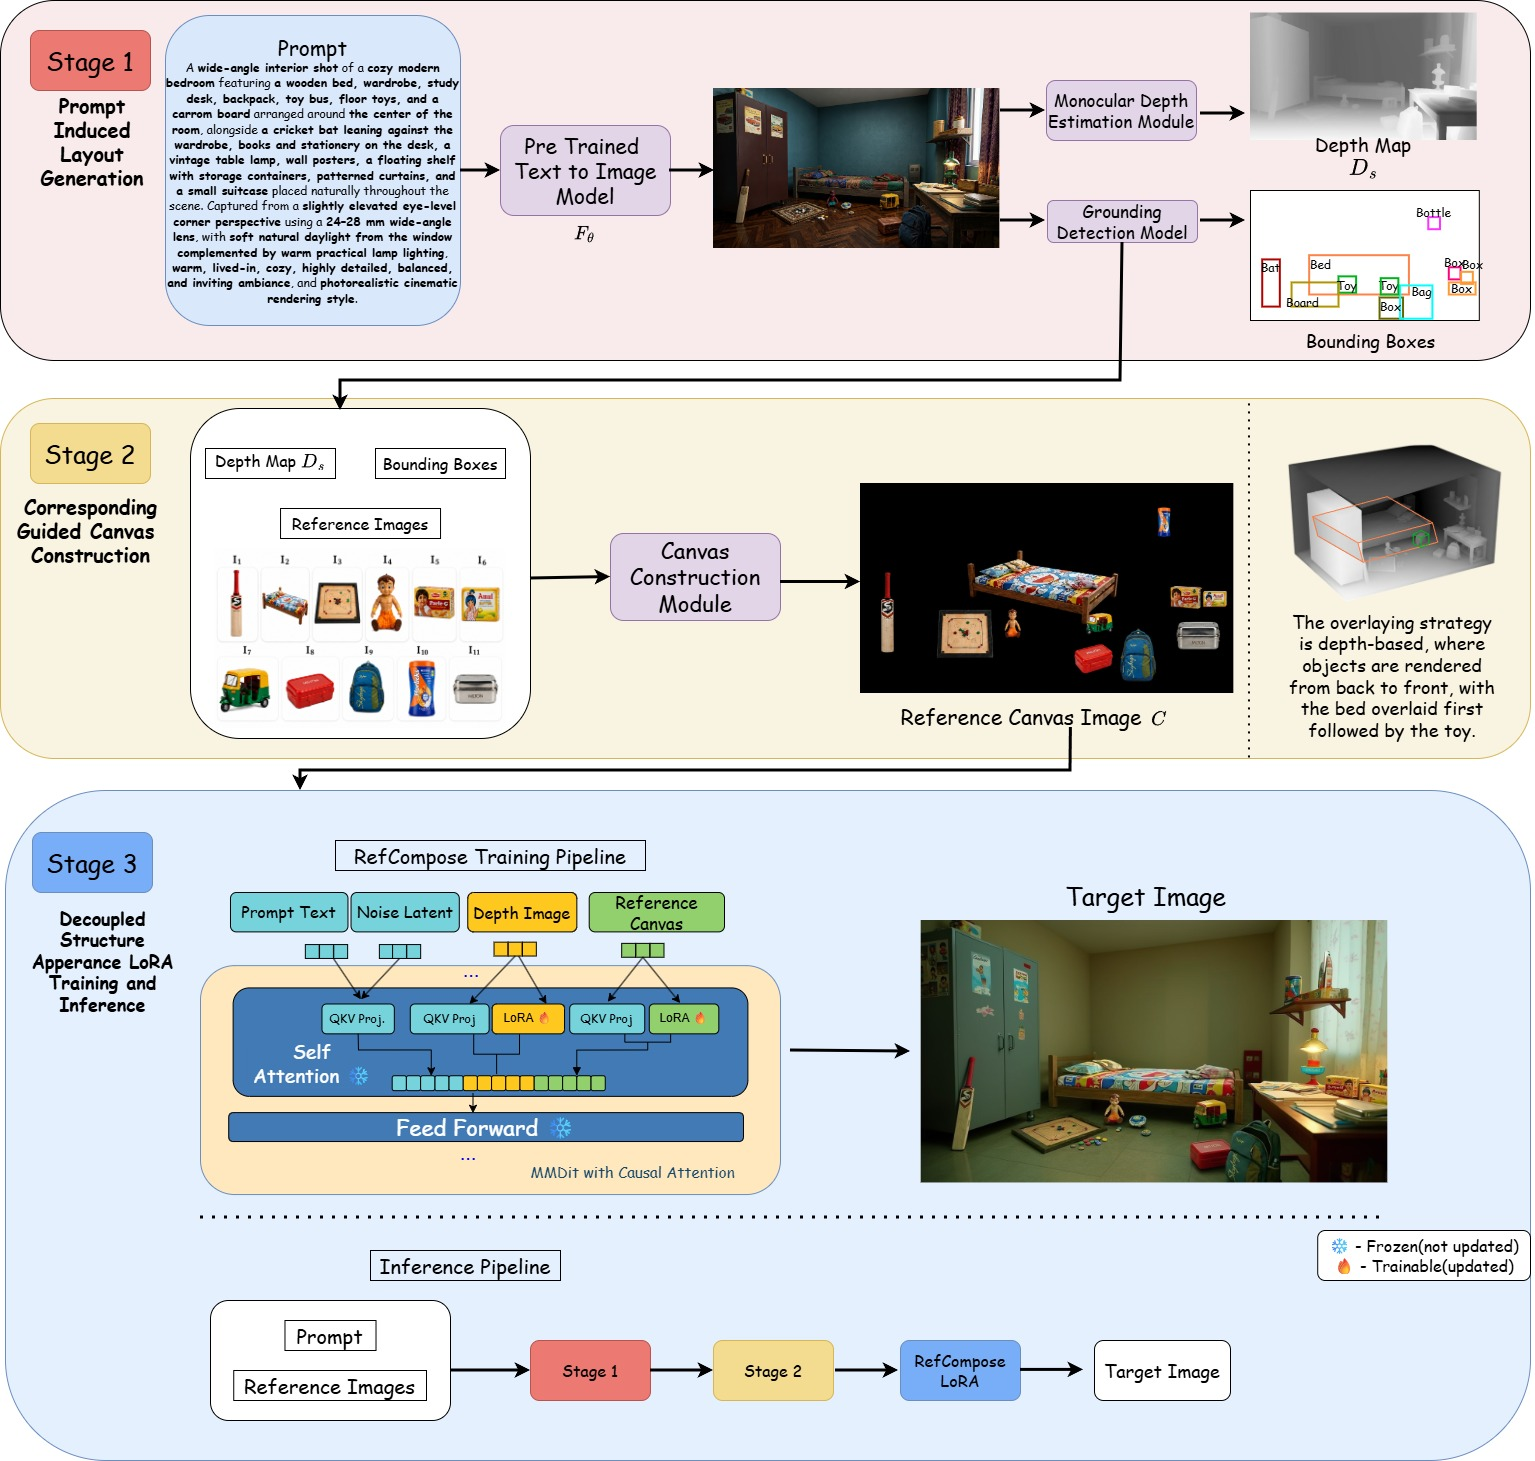
\includegraphics[width=\linewidth]{images/final_method.jpg}
\caption{End-to-end overview of the RefCompose pipeline across three stages: prompt-induced layout generation via a frozen diffusion transformer, correspondence-guided pixel-space canvas construction, and decoupled structure--appearance conditioning through dual LoRA streams within the MMDiT blocks. The depth map and reference canvas are injected through separate low-rank adaptation streams, ensuring structural and appearance signals remain disentangled throughout denoising. This design maintains constant token complexity irrespective of reference cardinality while preserving full-resolution subject identity.}
\label{fig:pipeline}
\end{figure}

Figure~\ref{fig:pipeline} summarises the pipeline.

\paragraph{Notation.}
Let $\mathcal{R} = \{I_1, \ldots, I_N\}$ denote the reference set of $N$ RGB images, $\mathbf{p}$ an object-centric structured prompt with explicit positional language, and $(H, W)$ the target output resolution.
The frozen pretrained diffusion transformer is $\mathcal{F}_\theta$; $\mathcal{E}$ and $\mathcal{E}^{-1}$ denote the VAE encoder and decoder respectively.

%----------------------------------------------------------
\subsection{Prompt-Induced Layout Generation}
\label{sec:layout}
%----------------------------------------------------------

Rather than querying an external layout model or LLM for bounding-box supervision, we exploit the spatial prior already internalised by a pretrained text-to-image transformer.
The prompt $\mathbf{p}$ is used primarily to describe the desired composition and spatial relationships among the referenced subjects; it does not need to encode their detailed appearance, because those cues are provided by the reference canvas.
A single generic composition prompt is sufficient in most cases, although users may add relational language for each subject (\emph{e.g.}, ``a person on the left, a product on the right'') when tighter placement control is needed.
A single forward pass of $\mathcal{F}_\theta$ then yields a coarse layout image:
%
\begin{equation}
  L = \mathcal{F}_\theta(\mathbf{p}) \in \mathbb{R}^{H \times W \times 3}.
\end{equation}
%
Modern diffusion transformers trained on web-scale corpora with strong text encoders have internalised rich statistical priors over spatial arrangement: relative scale, positional relationships, and object interaction are captured implicitly through cross-attention over token sequences.
% Box-level supervision is unnecessary; layout generation becomes a zero-cost byproduct of a standard generation call, eliminating LayoutGPT-style overhead entirely.
This approach provides a lightweight alternative to box-level supervision, as layout generation emerges naturally as a byproduct of a standard generation call, without requiring a dedicated layout model.

Bounding boxes are extracted from $L$ using Grounding DINO~\cite{liu2023grounding} as the grounding detector $\mathcal{G}$:
\begin{equation}
  \mathcal{B} = \mathcal{G}(L) = \{b_1, \ldots, b_N\}, \quad b_k = (x_k, y_k, w_k, h_k),
\end{equation}
where $b_k$ specifies the spatial region assigned to reference $I_k$ in the output frame.
These boxes serve as the spatial anchors for both canvas construction and depth estimation, ensuring that all downstream signals share a common spatial reference frame from the outset.

%----------------------------------------------------------
\subsection{Reference Canvas Representation}
%----------------------------------------------------------

With layout bounding boxes $\mathcal{B}$ established (Section~\ref{sec:layout}), we turn to the problem of encoding all $N$ references without incurring $\mathcal{O}(N)$ token growth.
Sequential encoding, which independently tokenises each reference and concatenates the resulting sequences, scales linearly with $N$ and forces the diffusion model to reconcile potentially incompatible token streams at every attention layer.
We replace this with a \emph{reference canvas} $\mathcal{C} \in \mathbb{R}^{H \times W \times 3}$: a fixed-resolution conditioning image in which each reference occupies the spatial region it is expected to cover in the output.
The image operation used to build this canvas is deliberately simple and standard; the role of the canvas is not to introduce a new compositing algorithm, but to convert a variable-cardinality reference set into a single spatially aligned conditioning signal.

Concretely, each reference $I_k$ is resized to the dimensions of its assigned box and pasted into the corresponding canvas region:
\begin{equation}
  \phi(I_k, b_k) = \mathrm{Resize}(I_k,\; h_k \times w_k)\;\text{placed at}\; b_k.
\end{equation}
When the boxes in $\mathcal{B}$ are pairwise disjoint, these patches are placed directly onto a blank canvas of size $H \times W$.
When boxes overlap, placement order must respect occlusion: the nearer reference must overwrite the farther one in the shared region.
Because overlap resolution depends on relative depth, the full canvas is assembled only after estimating a monocular depth map from the layout image $L$ (Section~\ref{sec:depth}).
The diffusion model receives a single spatially indexed conditioning image rather than $N$ independent token sequences.
The canvas is assembled in full pixel-space before any encoding, preserving fine-grained texture and identity details within each assigned region.

This representation yields the key scalability property: $\mathcal{C}$ is a \emph{single} image regardless of $N$, encoded once by the VAE:
\begin{equation}
  z_{\mathcal{C}} = \mathcal{E}(\mathcal{C}) \in \mathbb{R}^{(H/f) \times (W/f) \times c},
\end{equation}
where $f$ is the VAE spatial downsampling factor (typically $f = 8$) and $c$ is the latent channel dimension.
The canvas latent satisfies $|z_{\mathcal{C}}| = \text{const}$ for all $N$, directly contrasting with sequential schemes whose cost grows as $N \cdot (H/f)(W/f)c$.
This fixed-resolution conditioning eliminates the token explosion that afflicts concatenation baselines and caps GPU memory consumption at a hard ceiling independent of reference cardinality.

%----------------------------------------------------------
\subsection{Geometric Scaffolding via Depth Estimation}
\label{sec:depth}
%----------------------------------------------------------

Compositing references into a shared spatial frame is necessary but insufficient for geometric coherence.
Without an explicit structural prior, the diffusion model lacks information about depth ordering, surface orientation, and occlusion relationships, all of which govern the three-dimensional plausibility of the generated scene.
We therefore estimate a monocular depth map directly from the layout image:
\begin{equation}
  \mathcal{D}_s = \Psi(L) \in \mathbb{R}^{H \times W},
\end{equation}
where $\Psi$ denotes Depth Anything 3~\cite{depthanything3}, applied as a preprocessing step to the generated layout image.

Deriving $\mathcal{D}_s$ from $L$, rather than from the reference images themselves, is a deliberate design choice.
Because $L$, $\mathcal{B}$, and $\mathcal{D}_s$ all originate from the same layout image, they share an exact spatial reference frame.
Canvas region boundaries align with the depth map in image coordinates, and bounding boxes can be associated with depth-ordered object extents.
Since Depth Anything 3 is applied here to generated layouts rather than only to natural photographs, we treat its output as a relative geometric prior rather than metric ground truth; stylised layouts, ambiguous contact regions, and hallucinated object boundaries can induce local ordering errors.

The depth map also determines how overlapping canvas patches are layered.
For each reference $k$, we compute the mean depth within its box, $\bar{d}_k = \mathrm{mean}(\mathcal{D}_s \mid b_k)$, and sort references in descending order of $\bar{d}_k$ (far to near).
Let $\pi$ denote this permutation.
The reference canvas is then assembled by sequential overwrite compositing:
\begin{equation}
  \mathcal{C} =
  \mathrm{Paste}\!\left(
    \phi(I_{\pi(1)}, b_{\pi(1)}), \ldots,
    \phi(I_{\pi(N)}, b_{\pi(N)})
  \right),
\end{equation}
where $\mathrm{Paste}$ denotes placing the ordered patches onto a blank canvas and overwriting any pixels in the intersection with the newly added (nearer) reference.
Non-overlapping regions are unaffected by compositing order; in overlap regions, this depth-guided rule favours the subject estimated to be nearer and avoids requiring manual occlusion labels.
When the generated layout or monocular depth estimate produces an incorrect ordering, the resulting canvas can inherit that error, so the depth map is used as a practical ordering signal rather than an infallible occlusion oracle.

To make this structural signal compatible with the latent denoising process, $\mathcal{D}_s$ is encoded into the latent space via the VAE encoder $\mathcal{E}$:
\begin{equation}
  z_{\mathcal{D}} = \mathcal{E}(\mathcal{D}_s) \in \mathbb{R}^{h \times w \times c},
\end{equation}
where $z_{\mathcal{D}}$ carries the full geometric scaffold, including occlusion order, surface orientation, and spatial extent, in a latent representation commensurate with $z_{\mathcal{C}}$.


%----------------------------------------------------------
\subsection{Decoupled Structure--Appearance (DSA) LoRA}
%----------------------------------------------------------

Having constructed the depth latent $z_{\mathcal{D}}$ and the reference canvas latent $z_{\mathcal{C}}$, both signals must be injected into the frozen diffusion transformer without mixing their roles.
Naively concatenating them into a single conditioning stream allows depth features to influence appearance and vice versa, which can reduce the separation between structural and appearance cues.
We instead route each signal through a dedicated low-rank conditioning module, keeping structure and appearance streams disentangled throughout the denoising trajectory.

For a frozen projection matrix $W \in \mathbb{R}^{d_{\mathrm{out}} \times d_{\mathrm{in}}}$ inside the double-stream attention blocks, each LoRA branch learns a low-rank residual update
\begin{equation}
  \Delta W_m = B_m A_m, \qquad
  A_m \in \mathbb{R}^{r \times d_{\mathrm{in}}}, \quad
  B_m \in \mathbb{R}^{d_{\mathrm{out}} \times r}, \quad
  m \in \{s,a\},
\end{equation}
where $s$ denotes the structure branch conditioned on $z_{\mathcal{D}}$ and $a$ denotes the appearance branch conditioned on $z_{\mathcal{C}}$.
The effective projection is therefore $W + \Delta W_s + \Delta W_a$ for the conditioned layers, while the base parameters $W$ remain frozen.
Because Flux-style diffusion transformers are sampled with a flow-matching scheduler rather than a discrete DDPM reverse chain, we write the denoising process in scheduler-agnostic form.
Starting from the terminal latent $z_T$ drawn from the model prior, the sampler integrates the learned velocity field $v_\theta(z_t,t,\mathbf{p},z_{\mathcal{C}},z_{\mathcal{D}};\Delta W_s,\Delta W_a)$ over the scheduler time grid to obtain the clean latent:
\begin{equation}
  \hat{z}_0 = \mathcal{F}_\theta\!\left(\mathbf{p},\;z_T,\; z_{\mathcal{C}},\; z_{\mathcal{D}};\; \Delta W_s,\; \Delta W_a\right),
\end{equation}
where $\mathbf{p}$ provides semantic grounding, $z_{\mathcal{D}}$ enforces the geometric scaffold, and $z_{\mathcal{C}}$ grounds localised appearance. The synthesised output is recovered by VAE decoding:
\begin{equation}
  \hat{I} = \mathcal{E}^{-1}(\hat{z}_0) \in \mathbb{R}^{H \times W \times 3}.
\end{equation}




\section{Experiments}

\begin{figure}[t]
\centering
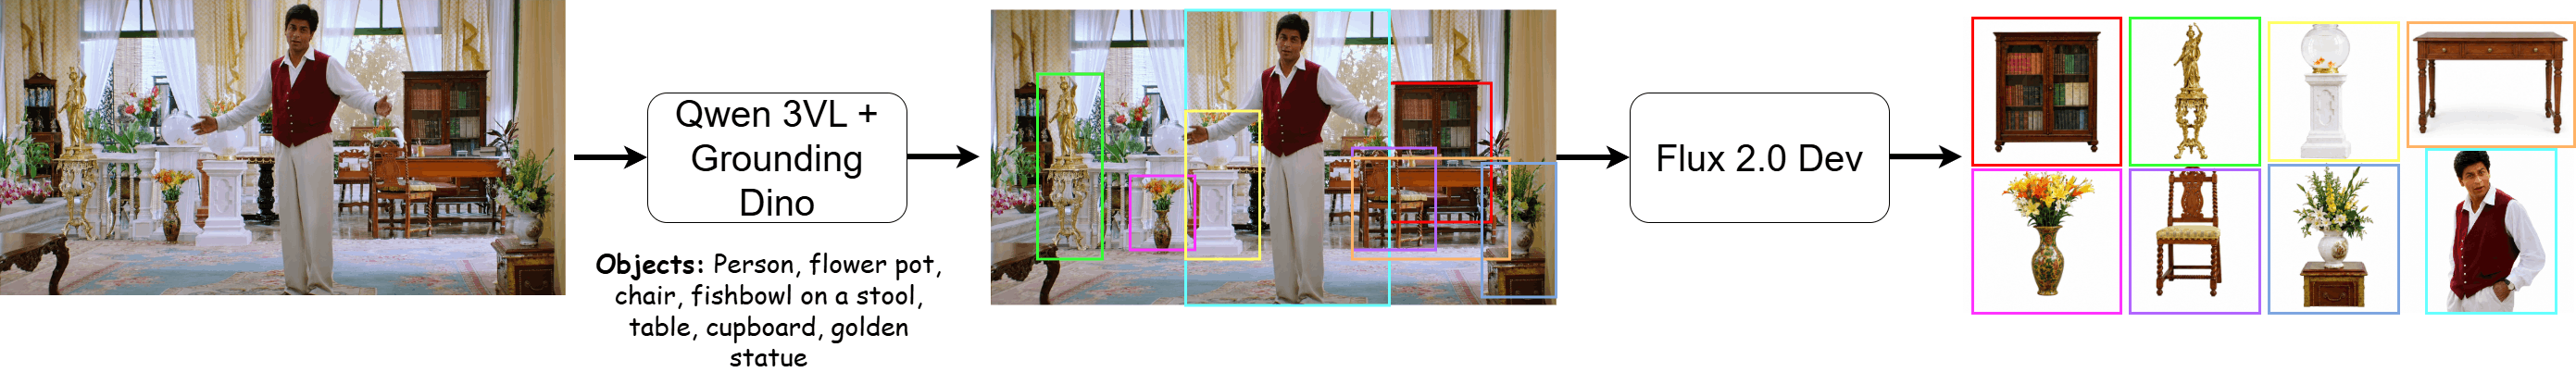
\includegraphics[width=\linewidth]{images/dataset_prep_compressed.png}
\caption{Overview of the dataset preparation pipeline. Movie shots are passed through Grounding DINO for object detection; detected crops are canonicalized with Flux~2.0 Dev to neutral pose and lighting; outputs are filtered by DINO similarity against the source crops; and retained samples are annotated with Qwen3-VL at both scene and crop level.}
\label{fig:data_pipeline}
\end{figure}

\subsection{Dataset Preparation}


\textbf{Dataset Construction.} We train on ultra high resolution cinematic imagery at $1280 \times 720$ resolution, drawn from Eros's proprietary movie catalogue, where most object references are canonicalized to a neutral pose. In addition, we construct a synthetic dataset using Flux 2.0 to complement this real data with diverse object positions and orientations, enabling the model to learn pose variation while the real dataset supplies richer textures; further details on its generation and composition are provided in the supplementary material.

Our data generation pipeline proceeds in four stages. First, each movie shot is passed through Grounding DINO~\cite{liu2023grounding} to detect candidate objects---actors, props, and landmarks---retaining only shots yielding more than four detected objects to ensure sufficient compositional density. Second, each detected object crop is fed to Flux~2.0 Dev to synthesize a neutral-pose, neutral-lighting canonicalization of the object, removing scene-specific pose and illumination variation. Third, we filter these canonicalized outputs against their original cropped counterparts using DINO cosine similarity, retaining a sample only if the similarity exceeds $0.90$; samples falling below this threshold are discarded as insufficiently faithful to the source reference. Finally, the retained shots are annotated using Qwen3-VL~\cite{qwen3vl}, producing both holistic scene-level descriptions and crop-level object descriptions, as illustrated in Figure~\ref{fig:data_pipeline}. This pipeline yields approximately $50{,}000$ samples drawn from $1{,}000$ distinct films from Eros's proprietary catalogue, together with additional samples generated through our synthetic dataset pipeline.


\subsection{Layout Generation}
\label{sec:layout-gen}

Given a set of $N$ reference subjects $\{I_1, \ldots, I_N\}$, the prompt is intended to provide the larger scene context and composition of the final image rather than the detailed appearance of each subject.
This differs from text-only generation: RefCompose already receives the visual content of the elements through the reference canvas, so the prompt mainly specifies how those elements should be arranged, what kind of scene they inhabit, and the desired camera or style context.
Consequently, no complex prompt-engineering rule is required in typical use, and generic scene-composition prompts are sufficient as long as they describe the desired spatial arrangement at a coarse level.
For consistency across experiments, we use the following template for RefCompose and all baselines, with bracketed slots filled from the reference set and scene metadata:
\begin{quote}
\small
\textit{A [shot type] of a [scene/environment] featuring [primary objects] arranged around [central subject], alongside [secondary objects/details] placed naturally throughout the scene. Captured from a [camera perspective] using a [lens type], with [lighting condition], [mood/style descriptors], and [photorealistic/cinematic rendering style].}
\end{quote}
The slots encode optional relational and positional language (\emph{e.g.}, primary objects and the central subject may be assigned left/right/foreground roles) when the desired composition requires it.
This prompt is passed to a frozen Flux~2.0 text-to-image diffusion transformer in a single forward pass to produce a coarse layout image $L$, from which bounding boxes $\{b_k\}_{k=1}^{N}$ are extracted using Grounding DINO~\cite{liu2023grounding}. No bounding-box supervision or auxiliary layout model is used in our pipeline; the spatial prior internalised by the transformer during large-scale pretraining provides a practical layout initialisation from text.

Because layout, object scale, and region extent are determined by the prompt and the resulting Flux~2.0 generation, the user can influence subject shape and size through shot type, relational placement, and scale descriptors in $\mathbf{p}$, which affect how $\mathcal{F}_\theta$ allocates canvas area across subjects.
When $N$ is large, each assigned region $b_k$ occupies a smaller fraction of the fixed $H \times W$ canvas, and $\mathrm{Resize}(I_k, h_k \times w_k)$ necessarily downsamples references into tighter patches.
This introduces within-canvas resolution degradation for individual subjects, independent of the constant token budget.
In practice, we mitigate this by specifying prominence and relative scale in the prompt so that critical references receive larger boxes in $L$.


\subsection{RefCompose LoRA}
We extend EasyControl~\cite{zhang2025easycontrol}'s Condition Injection LoRA to inject depth (structure) and a reference-canvas latent $z_{\mathcal{C}}$ (appearance) into a frozen Flux diffusion transformer through separate low-rank updates $\Delta W = BA$ with rank $r{=}32$ in the double-stream attention blocks; causal attention and KV caching keep the two streams disentangled, with the subject LoRA loaded before the depth LoRA at inference.
Training runs for $50{,}000$ iterations at $1280 \times 720$ in three stages while base weights remain frozen: ($1$) $10{,}000$ iterations on depth with a black canvas; ($2$) $20{,}000$ iterations with crops placed at Grounding DINO~\cite{liu2023grounding} boxes on the ground-truth image; ($3$) the remaining iterations with photometric jitter and mild spatial perturbations (affine warps, small translations) on crop placement to mimic inference-time misalignment between canvas and depth.
The first stage is used to initialise the structure branch before appearance cues are introduced; in early joint training without this warm-up, the model tends to use the canvas stream to compensate for geometry, reducing the separation between depth and appearance conditioning.
The second stage then teaches appearance grounding under clean placements, while the final perturbation stage improves robustness to the noisier boxes produced by the inference-time layout pipeline.
Because both branches condition on a single encoded canvas rather than per-reference token streams, GPU memory at inference stays approximately constant with reference count.

\paragraph{Evaluation benchmark.}
Quantitative and qualitative comparisons use the \emph{Dense Layout} test split introduced by InstanceAssemble~\cite{xiang2025instanceassemble}, which provides densely annotated multi-object scenes with ground-truth bounding boxes and per-instance text descriptions.
We adopt this benchmark to evaluate layout-aware composite generation under challenging many-object configurations; all reported metrics in Tables~\ref{tab:memory} and~\ref{tab:quant_results} are computed on this split unless stated otherwise.

\subsection{Quantitative Analysis}
\label{sec:quant}

\paragraph{Test set.}
Quantitative evaluation is performed on the Dense Layout test set of InstanceAssemble~\cite{xiang2025instanceassemble}, comprising $5{,}000$ composite targets held out from training.
Each example contains multiple objects with diverse subject categories (people, props, environments, and product-like assets).
On average, scenes contain $8.3$ annotated objects per image; we report aggregate means over the full test set in Table~\ref{tab:quant_results}.

\paragraph{Evaluation protocol and GPU memory.}

All methods are evaluated on a single NVIDIA H100 at \(1280 \times 720\) using the prompt template from Section~\ref{sec:layout-gen}. Following prior work, we select five object crops per image from the largest ground-truth boxes by area; each crop is passed through Flux~2.0 Dev to synthesize a neutral-pose, neutral-lighting canonicalization. Scene prompts are generated with Qwen3-VL~\cite{qwen3vl}, which fills the Section~\ref{sec:layout-gen} template with detailed scene context, object roles, and compositional language so that every method receives the same textual and visual information. These canonicalized reference images and prompts are fed to all multi-reference methods for the composite generation task. CreatiLayout and InstanceAssemble~\cite{xiang2025instanceassemble} receive only Dense Layout boxes and text, whereas UNO~\cite{wu2025uno}, XVerse~\cite{xverse2024}, and RefCompose additionally receive the same canonicalized reference crops. Region-wise metrics are computed using object localizations obtained from Grounding DINO~\cite{liu2023grounding}. As shown in Table~\ref{tab:memory}, token-based methods exhibit memory growth with increasing reference count and become out-of-memory at \(N=6\), while RefCompose maintains an approximately constant memory footprint through canvas compression. Consequently, all baseline comparisons are reported at \(N=5\), with Table~\ref{tab:quant_results} additionally reporting RefCompose in the \(N>5\) setting to demonstrate scalability to larger numbers of references without increasing memory usage.


Following LayoutSAM-Eval~\cite{xiang2025instanceassemble}, evaluation is divided into \emph{region-wise} and \emph{global-wise} quality. Region-wise metrics assess whether individual objects are generated at the correct locations and faithfully preserve the attributes specified by the input references and descriptions. Specifically, Spatial measures object placement accuracy, while Color, Texture, and Shape evaluate the fidelity of object appearance and structure. Global-wise metrics measure overall image quality, semantic consistency, and reference preservation. PICK and CLIP-T assess image-text alignment, DINO measures similarity to the target composition, DINO$_{\text{refs}}$ evaluates consistency with the supplied reference images, and CLIP-I captures image-level visual similarity. Higher values indicate better performance for all metrics.


\begin{table}[t]
  \centering
  \caption{Peak GPU memory (GB) at inference for varying reference count $N$ (batch size $1$; single H100; $1280 \times 720$).
  UNO~\cite{wu2025uno} and XVerse~\cite{xverse2024} are reference-image-based methods whose memory scales with the number of encoded references; both fail at $N{=}6$.
  RefCompose keeps memory approximately constant by canvas compression.
  OOM denotes out-of-memory failure.}
  \label{tab:memory}
  \setlength{\tabcolsep}{5pt}
  \begin{tabular}{lccc}
    \toprule
    \textbf{Method} & $N{=}2$ & $N{=}4$ & $N{=}6$ \\
    \midrule
    CreatiLayout~\cite{tang2024creatilayout} & 34.7 & 34.8 & 34.9 \\
    InstanceAssemble~\cite{xiang2025instanceassemble} & 35.2 & 35.3 & 35.4 \\
    UNO~\cite{wu2025uno} & 60.1 & 74.8 & OOM \\
    XVerse~\cite{xverse2024} & 59.6 & 75.3 & OOM \\
    \midrule
    \textbf{RefCompose} & \textbf{69.0} & \textbf{69.0} & \textbf{69.0} \\
    \bottomrule
  \end{tabular}
\end{table}

\begin{table*}[!t]
  \centering
  \caption{Quantitative comparison on the Dense Layout test set~\cite{xiang2025instanceassemble} ($5{,}000$ images; mean $8.3$ objects per image).
  Previous methods use five references per example because UNO and XVerse are not runnable beyond this setting on one H100; the $N{>}5$ RefCompose row evaluates the same model with additional references.
  Higher is better for all metrics.
  Reported values are means over the test set.
  \textbf{Bold} denotes the best overall result; the improvement row compares RefCompose ($N{>}5$) only against the strongest reference-image baseline for each metric.}
  \label{tab:quant_results}
  \resizebox{\textwidth}{!}{%
  \setlength{\tabcolsep}{8pt}
  \begin{tabular}{lccccccccc}
    \toprule
    {\textbf{Method}}
    & \multicolumn{4}{c}{\textbf{Region-wise Quality}}
    & \multicolumn{5}{c}{\textbf{Global-wise Quality}} \\
    \cmidrule(lr){2-5} \cmidrule(lr){6-10}
    & \textbf{Spatial}$\uparrow$
    & \textbf{Color}$\uparrow$
    & \textbf{Texture}$\uparrow$
    & \textbf{Shape}$\uparrow$
    & \textbf{PICK}$\uparrow$
    & \textbf{DINO}$\uparrow$
    & \textbf{DINO$_{\text{refs}}$}$\uparrow$
    & \textbf{CLIP-I}$\uparrow$
    & \textbf{CLIP-T}$\uparrow$ \\
    \midrule
    \multicolumn{10}{l}{\textit{Layout-only baselines}} \\
    CreatiLayout~\cite{tang2024creatilayout}
      & 0.726 & 0.487 & 0.518 & 0.501
      & 0.222 & 0.696 & 0.482 & 0.727 & \textbf{0.335} \\
    InstanceAssemble~\cite{xiang2025instanceassemble}
      & 0.790 & 0.590 & 0.620 & 0.610
      & 0.221 & 0.686 & 0.457 & 0.703 & 0.330 \\
    \midrule
    \multicolumn{10}{l}{\textit{Reference-image baselines}} \\
    UNO~\cite{wu2025uno}
      & 0.750 & 0.500 & 0.530 & 0.520
      & 0.225 & 0.821 & 0.548 & 0.742 & 0.329 \\
    XVerse~\cite{xverse2024}
      & 0.665 & 0.421 & 0.442 & 0.428
      & 0.218 & 0.686 & 0.506 & 0.731 & 0.302 \\
    \midrule
    \textbf{RefCompose} ($N{=}5$)
      & 0.908 & 0.826 & 0.854 & 0.849
      & 0.229 & 0.959 & 0.613 & 0.766 & 0.327 \\
    \textit{vs. best reference baseline}
      & \textcolor{green!60!black}{+0.172}
      & \textcolor{green!60!black}{+0.338}
      & \textcolor{green!60!black}{+0.336}
      & \textcolor{green!60!black}{+0.341}
      & \textcolor{green!60!black}{+0.006}
      & \textcolor{green!60!black}{+0.150}
      & \textcolor{green!60!black}{+0.077}
      & \textcolor{green!60!black}{+0.036}
      & 0.000 \\
    \textbf{RefCompose} ($N{>}5$)
      & \textbf{0.922} & \textbf{0.838} & \textbf{0.866} & \textbf{0.861}
      & \textbf{0.231} & \textbf{0.971} & \textbf{0.625} & \textbf{0.778} & 0.329 \\
    \bottomrule
  \end{tabular}%
  }
\end{table*}

\begin{figure}[t]
\centering
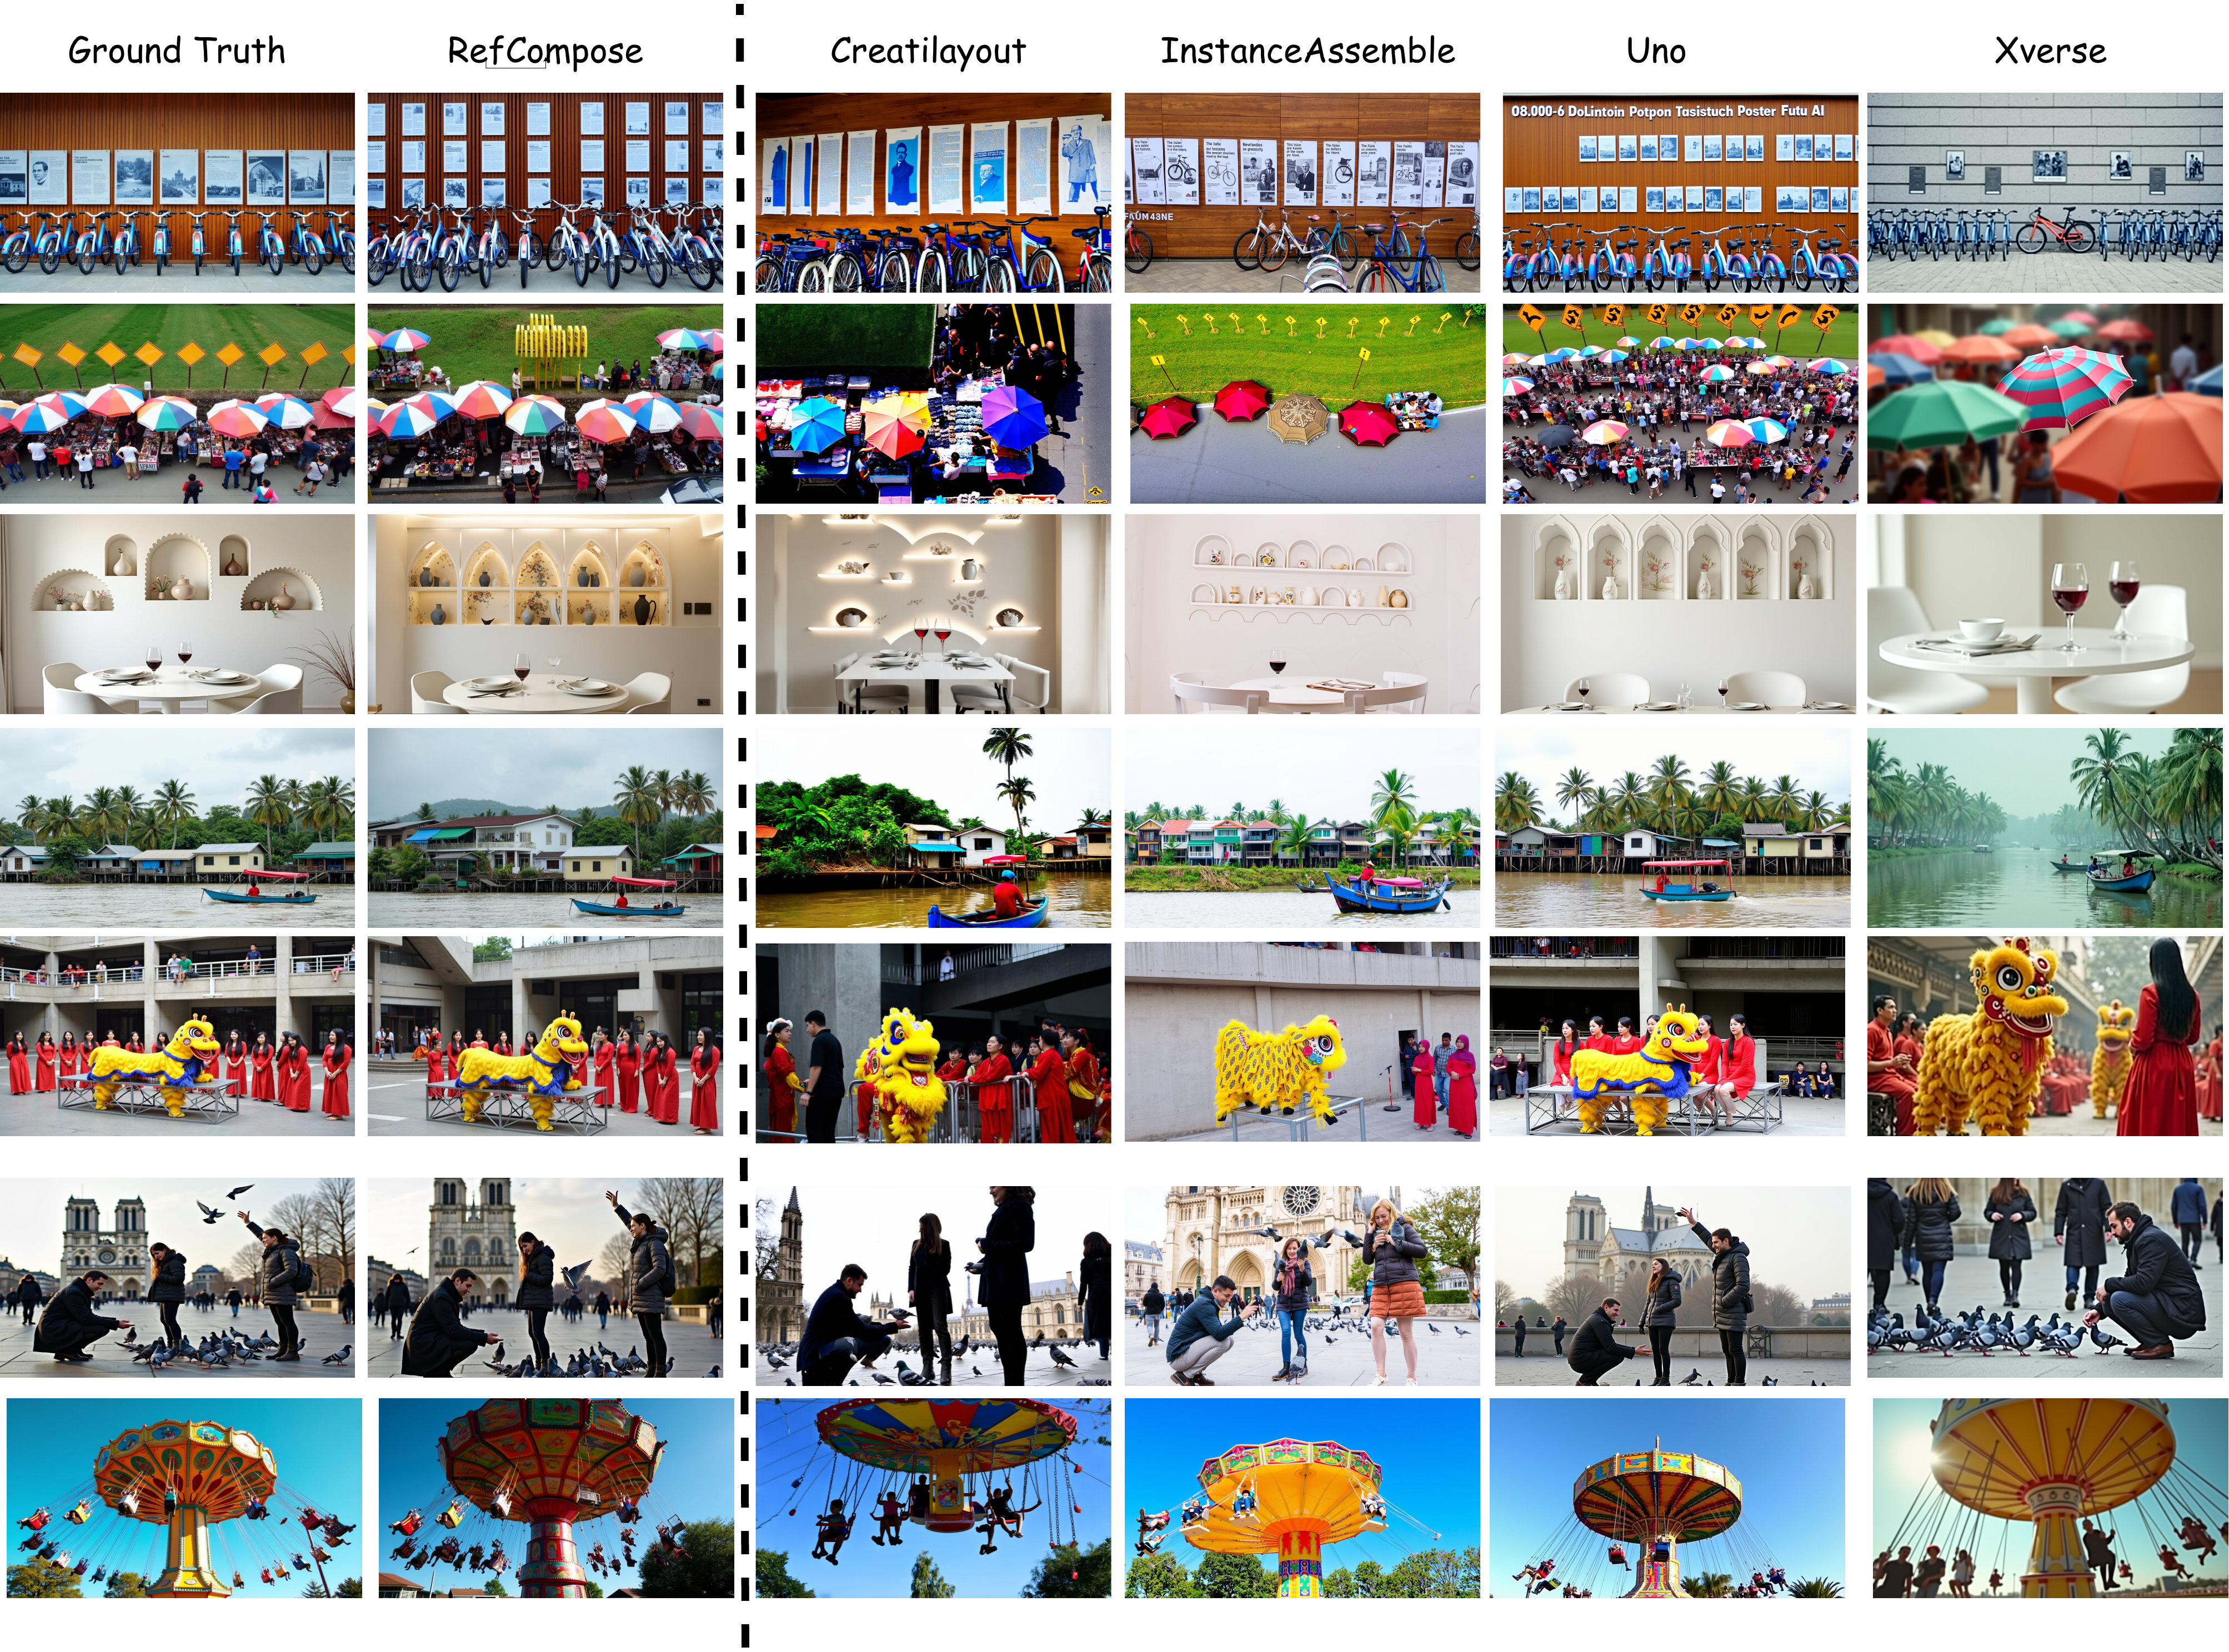
\includegraphics[width=\linewidth]{images/qual.png}
\caption{Qualitative comparison of RefCompose against CreatiLayout, InstanceAssemble, UNO, and XVerse across seven diverse multi-subject scenes, with ground truth in the leftmost column. Layout-conditioned baselines hallucinate subject appearance while token-based methods exhibit subject drift and loss of fine-grained detail under multi-object compositions. RefCompose consistently reproduces both spatial arrangement and photometric identity with the highest fidelity across all scene types.}
\label{fig:teaser}
\end{figure}

Layout-conditioned baselines (CreatiLayout, InstanceAssemble) operate without visual reference input, so photometric metrics primarily measure the value of reference conditioning; comparisons against UNO~\cite{wu2025uno} and XVerse~\cite{xverse2024} provide the more architecturally matched evaluation.

% \paragraph{Comparison to token-based reference methods.}
% Relative to UNO~\cite{wu2025uno} and XVerse~\cite{xverse2024}, the most direct reference-image-based baselines, RefCompose improves spatial accuracy ($0.908$ vs.\ $0.750$ and $0.665$), colour ($0.826$ vs.\ $0.500$ and $0.421$), texture ($0.854$ vs.\ $0.530$ and $0.442$), and shape ($0.849$ vs.\ $0.520$ and $0.428$) under the matched five-reference protocol.
% RefCompose also attains higher DINO ($0.959$) and DINO$_\text{refs}$ ($0.613$ vs.\ $0.548$ and $0.506$), indicating stronger semantic and identity alignment to both the composite target and the supplied references.
% Table~\ref{tab:quant_results} therefore reports improvement margins only against the strongest reference-image baseline for each metric.
% These gains coincide with the memory profile in Table~\ref{tab:memory}: token concatenation incurs linear GPU growth and fails at $N{=}6$ on a single H100, whereas canvas conditioning keeps memory approximately flat.
% UNO remains competitive on CLIP-I ($0.742$) and PICK ($0.225$), reflecting partial appearance transfer despite weaker spatial localisation in the evaluated multi-object setting.

\paragraph{Comparison to token-based reference methods.}
RefCompose consistently outperforms token-based reference methods such as UNO~\cite{wu2025uno} and XVerse~\cite{xverse2024}, achieving higher spatial accuracy (0.908 vs.\ 0.750), colour fidelity (0.826 vs.\ 0.500), and reference alignment (DINO$_\text{refs}$: 0.613 vs.\ 0.548). Moreover, canvas conditioning maintains an approximately constant memory footprint, whereas token-concatenation approaches scale linearly with the number of references. These results highlight the effectiveness of decoupling appearance and layout cues for multi-object reference-conditioned generation.



\paragraph{Comparison to layout-conditioned methods.}
% Within the layout-only group, CreatiLayout and InstanceAssemble achieve strong text-alignment scores, with CreatiLayout obtaining the highest CLIP-T score ($0.335$), and InstanceAssemble reaches the higher spatial score ($0.790$), confirming that explicit box supervision aids placement even without reference pixels.
% Their substantially lower colour, texture, and shape scores are expected given that they must hallucinate appearance from text; these metrics should be read as characterising the value of reference conditioning, not as a like-for-like architectural comparison.
% RefCompose's lead on photometric and DINO$_\text{refs}$ metrics is most meaningful when contrasted with UNO and XVerse, which receive the same reference crops under the same memory-bounded regime.
Within the layout-only group, CreatiLayout and InstanceAssemble achieve strong 
text-alignment scores, with CreatiLayout obtaining the highest CLIP-T score 
($0.335$) and InstanceAssemble achieving the higher spatial score ($0.790$), 
confirming that explicit box supervision aids placement even without reference 
pixels. Their substantially lower colour, texture, and shape scores reflect the 
information loss due to the absence of reference pixels rather than an architectural 
limitation, as these methods derive appearance entirely from text. RefCompose's 
photometric and DINO$_\text{refs}$ gains are therefore best evaluated against UNO 
and XVerse, which operate under the same memory-bounded regime with identical 
reference crops.

\paragraph{Global preference and text alignment.}
PICK scores are comparatively tight, ranging from $0.218$ (XVerse) to $0.229$ (RefCompose), so the larger separations on spatial, photometric, and DINO$_\text{refs}$ metrics are more informative for this task.
RefCompose obtains a CLIP-T score of $0.327$, slightly below UNO ($0.329$) and the layout-conditioned baselines, indicating that text-only alignment is complementary rather than the primary indicator of reference-grounded composition quality.


\subsection{Qualitative Analysis}
Figure~\ref{fig:teaser} corroborates the quantitative trends across seven multi-subject scenes.
CreatiLayout and InstanceAssemble place objects coherently from boxes and text but hallucinate colour, texture, and identity, especially for distinctive materials where language is a poor substitute for pixels.
UNO~\cite{wu2025uno} and XVerse~\cite{xverse2024} transfer some reference appearance yet show subject drift and softened fine detail under multi-object layouts in our qualitative examples.
RefCompose composites references at full resolution on a shared canvas and conditions denoising with an aligned depth map, yielding subjects at correct locations with faithful photometric detail; overlapping instances are best separated where depth discontinuities match canvas boundaries and the dual LoRA streams limit cross-region leakage.
The lower CLIP-T score relative to layout-conditioned baselines reflects an expected tradeoff: canvas conditioning can shift generation toward reference fidelity at a minor cost to global text alignment, so spatial and DINO$_\text{refs}$ metrics are more diagnostic for reference-grounded composition.
Residual failures appear when prompt-induced layouts imply ambiguous occlusion or implausible depth, which bounds geometric plausibility even though the depth prior corrects most floating and interpenetration artefacts relative to layout-only baselines.

\paragraph{Multi-reference flexibility.}
Figure~\ref{fig:multi_reference} evaluates two distinct reference sets for the same scene configuration.
A Flux~2.0-generated layout image defines where each subject should appear, while the estimated depth map supplies additional geometric cues for relative orientation and placement.
By conditioning jointly on the reference canvas and depth prior, RefCompose synthesises coherent outputs for both reference sets, preserving the intended spatial arrangement while transferring the appearance of each supplied subject.

\begin{figure}[t]
\centering
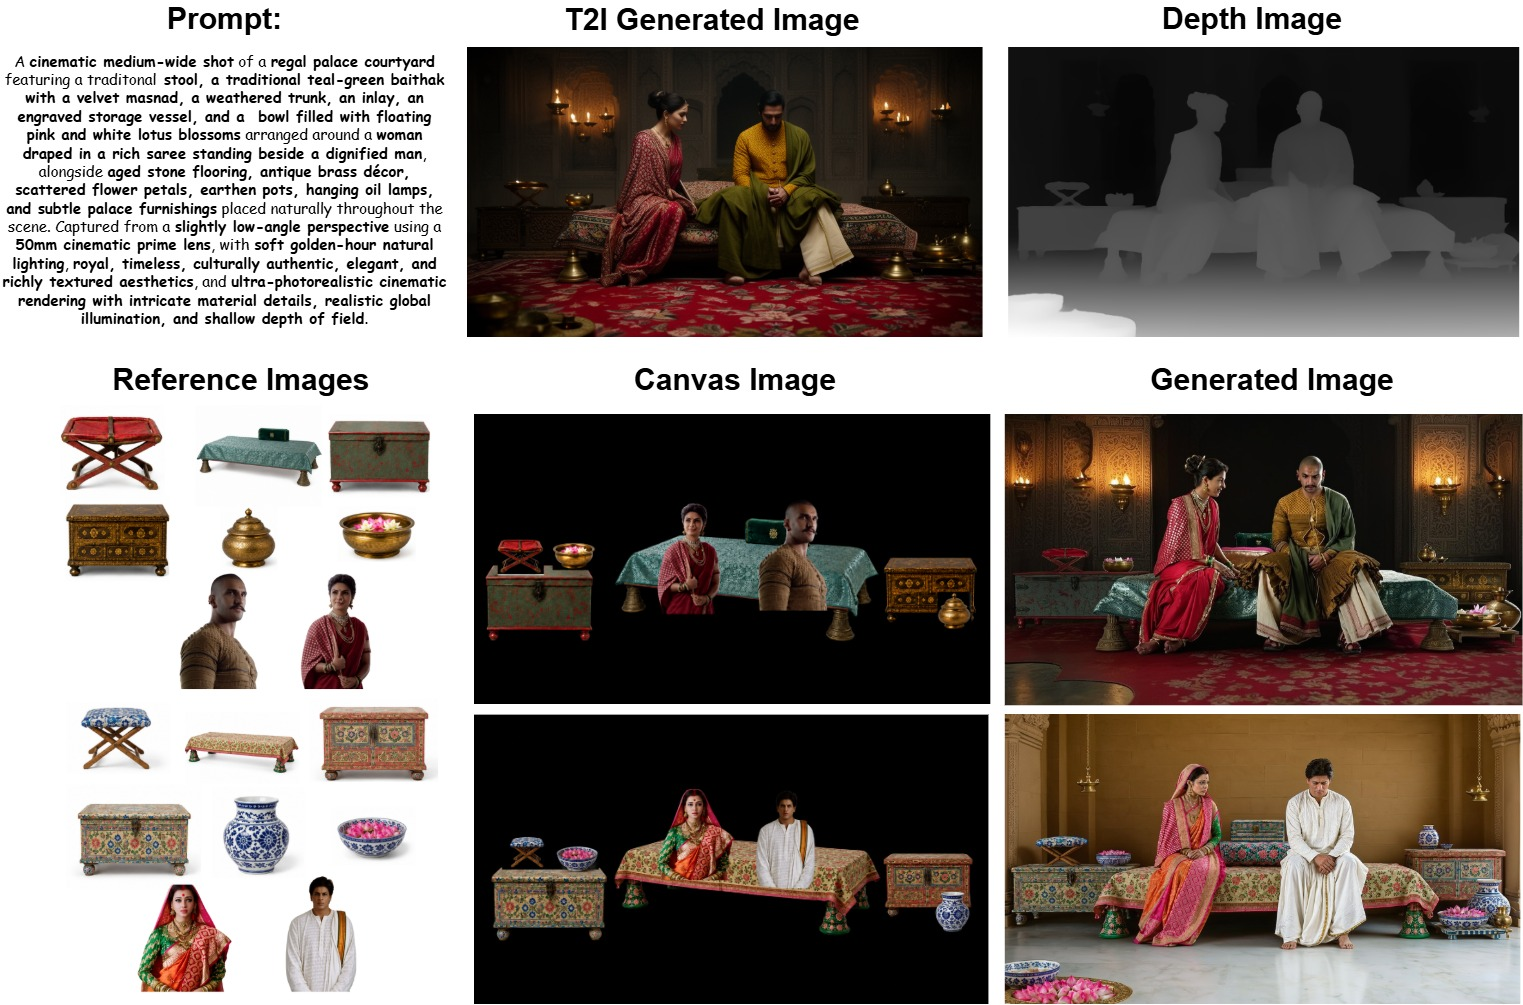
\includegraphics[width=\linewidth]{images/multi_reference_images.jpg}
\caption{Qualitative example with two different reference sets for the same scene layout. The prompt-induced canvas and aligned depth map provide shared structural priors, while the reference images specify subject appearance. RefCompose generates semantically consistent composites for both reference configurations.}
\label{fig:multi_reference}
\end{figure}

\paragraph{Depth-controlled orientation.}
Figure~\ref{fig:orientation_control} further isolates the role of the depth prior by holding the reference assets fixed and varying only the depth map.
In the first example, the depth map describes a conventional arrangement in which objects are naturally placed around a sweet shop.
In the second, the depth map is edited to depict a dynamic scene with floating debris, airborne bricks, and scattered objects.
Despite identical reference inputs, the generated results follow the geometry and orientation encoded by each depth map, demonstrating that RefCompose can control scene dynamics and spatial arrangement while preserving reference identity.

\begin{figure}[t]
\centering
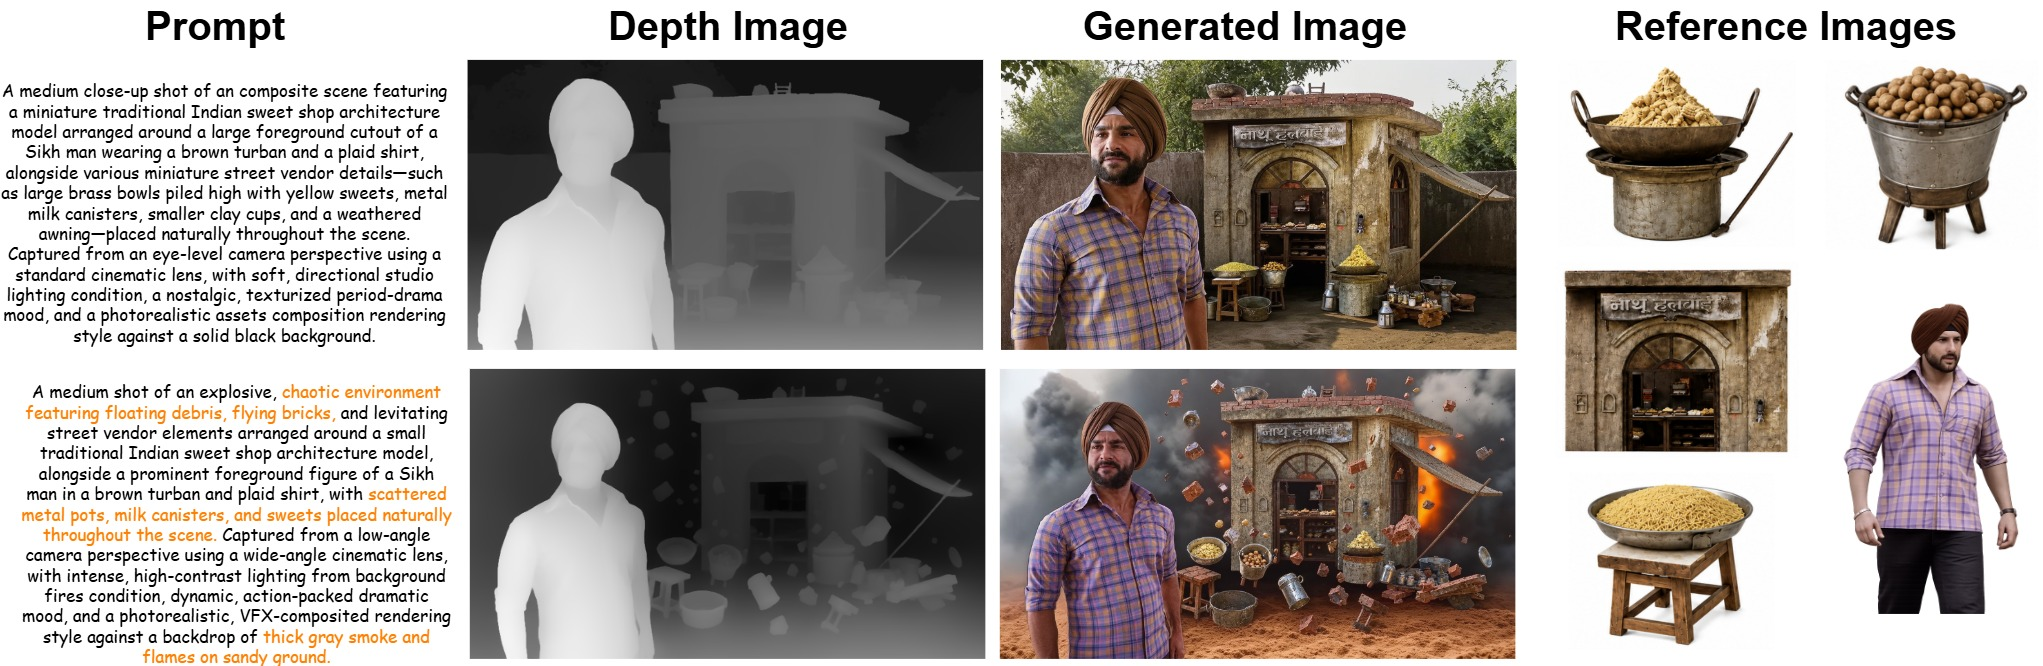
\includegraphics[width=\linewidth]{images/orientation_picture.jpg}
\caption{Depth-controlled generation with identical reference assets. Changing only the depth map alters object orientation and scene dynamics---from a static sweet-shop arrangement to a chaotic environment with floating debris---while reference appearance remains stable.}
\label{fig:orientation_control}
\end{figure}


\subsection{Ablation Study}
\label{sec:ablation}

Figure~\ref{fig:ablation} ablates the reference canvas and depth prior on an indoor multi-object scene (reference crops shown below).

\begin{figure}[!tb]
\centering
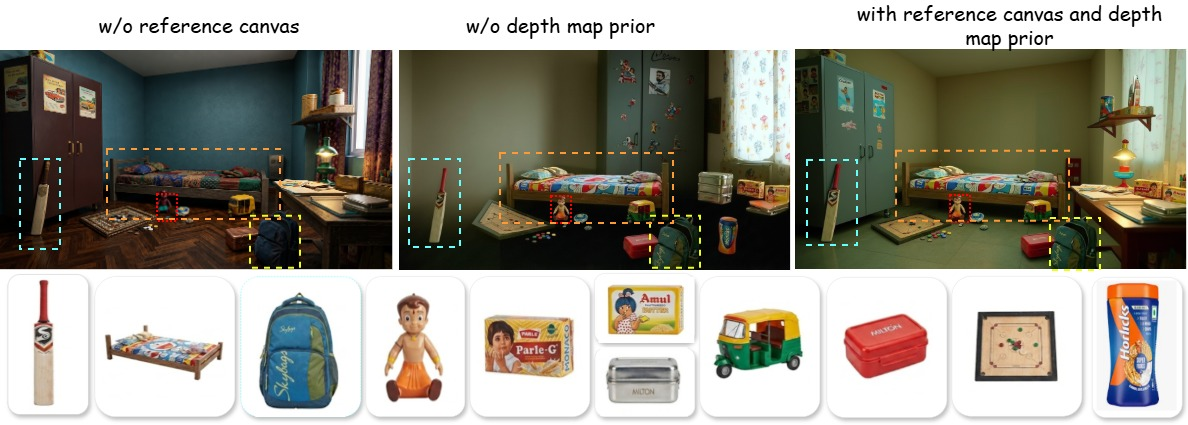
\includegraphics[width=\linewidth]{images/final_abalation.jpg}
\caption{Ablation study isolating the contributions of the reference canvas and depth map prior on an indoor multi-object scene, with corresponding input reference crops shown below. Removing either component individually degrades subject identity or geometric coherence, manifesting as hallucinated textures or incorrect spatial placement respectively. The full model combining both conditioning signals achieves accurate appearance preservation and geometrically consistent composition, confirming their complementary necessity.}
\label{fig:ablation}
\end{figure}

Removing the canvas forces the model to infer appearance solely from textual descriptions, resulting in plausible scene layouts but hallucinated object colours, textures, and identities. As illustrated by the bag and toy examples, the depth prior effectively constrains object layout and spatial positioning, yet fails to transfer the appearance characteristics specified by the reference images. Conversely, removing the depth signal preserves partial appearance transfer but degrades spatial reasoning, leading to incorrect object placement and occlusion relationships. For example, although the bat and bed remain recognizable, their arrangement is contextually implausible and fails to reflect realistic object interactions. In contrast, the full model leverages both canvas and depth cues from the same layout frame through decoupled LoRA streams, simultaneously preserving subject appearance and geometric consistency. These results demonstrate that canvas and depth provide complementary information, with appearance and structure jointly contributing to high-fidelity scene generation.

\FloatBarrier
\section{Conclusion}

% This work addresses multi-reference image generation under fixed memory cost, where token-concatenation and QKV-injection approaches struggle to preserve appearance fidelity and spatial precision as the number of references grows. 
% This work addresses multi-reference image generation under a fixed memory cost, where token concatenation and QKV injection approaches struggle to preserve appearance fidelity and spatial precision, and text-only conditioning fails to maintain cultural and ethnic fidelity as the number of references and scene heterogeneity grow.
% RefCompose introduces a pixel-space compositional conditioning framework that encodes an arbitrary number of reference images onto a single fixed-resolution canvas, decoupling token complexity from reference cardinality. Spatial layout is induced from a structured text prompt through a frozen diffusion transformer, with Grounding DINO used to extract boxes from the generated layout rather than relying on annotated training boxes or a dedicated layout-generation model. A dual-stream LoRA injects depth and appearance signals through disentangled low-rank adaptation paths, enforcing geometric consistency and subject identity simultaneously. Quantitative evaluation shows gains over the strongest reference-image baseline in the $N{>}5$ setting, including $+0.172$ spatial accuracy, $+0.077$ DINO$_\text{refs}$, and $+0.036$ CLIP-I, while keeping inference memory constant with respect to reference count.
This work addresses multi-reference image generation under a fixed memory cost, 
where token concatenation and QKV injection approaches struggle to preserve 
appearance fidelity and spatial precision, and text-only conditioning fails to 
maintain cultural and ethnic fidelity as the number of references and scene 
heterogeneity grow. RefCompose introduces a pixel-space compositional conditioning 
framework that encodes an arbitrary number of reference images onto a single 
fixed-resolution canvas, decoupling token complexity from reference cardinality. 
Spatial layout is induced from a structured text prompt through a frozen diffusion 
transformer, with Grounding DINO used to extract boxes from the generated layout 
rather than relying on annotated training boxes or a dedicated layout-generation 
model. A dual-stream LoRA injects depth and appearance signals through disentangled 
low-rank adaptation paths, enforcing geometric consistency and subject identity 
simultaneously. Quantitative evaluation demonstrates that RefCompose consistently 
outperforms reference-image baselines across appearance fidelity and spatial accuracy 
metrics, while maintaining constant inference memory regardless of reference count.

\section{Limitations}

RefCompose depends on a chain of upstream components, including prompt-induced layout $L$, Grounding DINO localisation, and a Depth Anything~3 map, whose errors compound when the structured template (Section~\ref{sec:layout-gen}) is ambiguous, when detections are missed or misaligned on generated images, or when monocular depth mis-orders overlapping regions on synthetic layouts.
Although canvas encoding avoids linear token growth with $N$, each reference is still resized to a fixed $H \times W$ patch, so large object counts or small assigned boxes attenuate fine-grained identity before encoding, and viewpoint mismatch between $L$ and the reference crops (e.g., bird's-eye depth with lateral portraits) can yield contradictory depth and appearance cues.
Our quantitative study caps previous methods at five references for fair comparison with memory-limited baselines, while reporting an additional RefCompose-only $N{>}5$ setting.



\bibliographystyle{splncs04}
\bibliography{main}
\end{document}
